\chapter{Проектирование приложения для общего списка дел}

\section{Предметная область и назначение программы}

Списки дел используются для записи учебных заданий, покупок, личных планов и других предстоящих дел. Для каждой задачи хранятся идентификатор, название и отметка выполнения. Например, задачу «Сдать практическую работу» можно добавить в общий перечень и отметить выполненной после завершения. Даты, приоритеты, категории и повторяющиеся события в рассматриваемую модель не входят. Для двух компьютеров достаточно общего перечня задач и отметок об их выполнении.

Пользователь может работать на двух компьютерах. При локальном хранении на каждом устройстве возникли бы два независимых списка. Даже если файлы имеют одинаковую структуру, они со временем расходятся: на одном компьютере задача отмечена выполненной, а на втором об этом ещё неизвестно. При ручном копировании файлов нужно отдельно следить, какая версия списка последняя. Список хранится в SQLite на первом компьютере; оба клиента обращаются к нему через FastAPI.

Приложение рассчитано на локальную сеть, например домашнюю или учебную. Один компьютер запускает сервер и хранит данные. Второй компьютер является клиентом. При этом на первом компьютере тоже можно запустить клиент, поэтому у обоих пользователей будет одинаковый интерфейс. Сведения о задачах передаются по HTTP в виде JSON-документов. Клиент отправляет запрос, сервер возвращает ответ; такой обмен описан в русскоязычном руководстве MDN \cite{mdnhttp}. JSON представляет данные в виде объектов, массивов и значений разных типов \cite{rfcjson}. В ответе сервера передаются идентификатор, название и состояние задачи.

Основу серверного интерфейса составляют чтение списка, добавление записи, исправление её названия, переключение отметки и удаление. После каждой операции данные остаются в одной базе. Сервер отвечает за проверку запроса и изменение нужной строки, а клиенты - за отображение результата. Такой способ хранения позволяет работать с задачами по идентификатору, даже если две записи имеют одинаковое название.

Сохранение данных и синхронизация проверяются раздельно. Сохранение означает, что запись остаётся в SQLite после перезапуска сервера. Синхронизация означает, что изменение с одного компьютера получает второй клиент. Если задача видна на другом ПК, но исчезает после перезапуска сервера, обмен данными работает, а сохранение данных не работает. Поэтому отдельно проверяются чтение общей базы и повторный запуск с тем же файлом данных.

У программы есть несколько допущений. Компьютеры используют доверенную локальную сеть; в приложении нет личных аккаунтов. Пользователи видят один список, а не личные списки каждого. Клиенты подключаются к серверу по его локальному IP-адресу. Если компьютер-сервер выключен, клиент сохраняет на экране ранее полученный список, но не обновляет его. Нижняя строка сообщает об отсутствии связи; отправка новой команды завершится ошибкой.

\section{Пользовательские действия и требования}

Функции приложения определены по последовательности действий пользователя. При составлении требований учитываются действия, исходные данные и ожидаемый результат операции; такой способ описания используется при проектировании информационных систем \cite{zaramenskikh,chistov}. После открытия приложения пользователь видит список задач. Он может создать новую запись, исправить название, отобрать записи по тексту или состоянию, а также отметить выполнение. Для удаления требуется выбрать конкретную строку. Второй компьютер должен показывать тот же перечень, хотя обновление может произойти с небольшой задержкой. Эти действия сформировали набор функциональных требований, приведённый в таблице \ref{tab:req-functional}.

\begin{table}[H]
\caption{Функциональные требования к приложению}
\label{tab:req-functional}
\small\centering\renewcommand{\arraystretch}{1.25}
\begin{tabularx}{\textwidth}{|L{13mm}|Y|L{33mm}|}
\hline
Код & Требование & Проверяемый результат \\
\hline
F1 & Показать актуальный перечень задач & Виден список записей \\
\hline
F2 & Добавить задачу с непустым названием & Новая запись появилась \\
\hline
F3 & Изменить отметку о выполнении & Состояние поменялось \\
\hline
F4 & Удалить выбранную задачу & Запись исчезла \\
\hline
F5 & Передать изменения второму клиенту & Список на ПК №2 обновился \\
\hline
F6 & Сохранить задачи после перезапуска & Список остался в базе \\
\hline
F7 & Обработать неверный ввод & Ошибочная запись не создана \\
\hline
F8 & Показать проблему соединения & Пользователь видит сообщение \\
\hline
F9 & Перейти между тремя страницами & Переключается раздел интерфейса \\
\hline
F10 & Исправить название существующей задачи & Новое название сохранено \\
\hline
F11 & Найти задачи и применить фильтр & Видны подходящие записи \\
\hline
F12 & Посчитать выполненные задачи & Показаны числа и процент \\
\hline
F13 & Сохранить список в TXT & Создан текстовый файл со всеми задачами \\
\hline
\end{tabularx}
\end{table}

Ввод названия задачи ограничен 120 символами. То же правило действует при редактировании. Сервер проверяет текст независимо от клиентского окна, поскольку запрос можно отправить и напрямую через страницу документации API. Название проверяется после удаления пробелов по краям строки; длина должна составлять от 1 до 120 символов. Управляющие символы (например, перевод строки и табуляция) сервер отклоняет: название должно отображаться одной строкой списка \cite{owaspvalidation}.

Признак выполнения принимает два значения. В интерфейсе выполненная задача отмечается знаком [x], невыполненная: знаком [ ]; при передаче по сети используется логическое значение. В списке не нужно выводить техническое значение поля \texttt{done}. Название записи остаётся одинаковым независимо от состояния. Повторное изменение переводит задачу из состояния «Выполнено» обратно в «В работе».

При редактировании название меняется только у выбранной записи; её идентификатор и отметка выполнения сохраняются. Поиск и фильтрация выполняются над уже полученным списком на клиенте и не изменяют содержимое базы данных. Кнопка «Сохранить в TXT» записывает все задачи в текстовый файл на компьютере пользователя; отдельный маршрут на сервере для этого не нужен. Для удаления пользователь должен выбрать строку списка. Если ни одна строка не выбрана, интерфейс показывает подсказку. На уровне сервера удаление выполняется по идентификатору. Когда такого идентификатора нет, сервер отвечает кодом 404, не изменяя другие записи. Это позволяет отделить отсутствие задачи от успешно проведённой операции. Семантика ошибок HTTP и назначение кодов ответа описаны в стандарте HTTP \cite{rfchttp}.

Нефункциональные требования касаются установки, работы с сетью и отображения ошибок. Программа должна запускаться без внешней учётной записи, а для хранения данных не должна требоваться установка отдельного серверного процесса базы данных. Все основные действия располагаются в одном окне. Для всех сетевых запросов установлен тайм-аут 2 секунды. Запросы выполняются в графическом потоке, поэтому при задержке сети окно может на короткое время перестать отвечать. Перечень нефункциональных требований приведён в таблице \ref{tab:req-nonfunctional}. 

\begin{table}[H]
\caption{Нефункциональные требования и ограничения}
\label{tab:req-nonfunctional}
\small\centering\renewcommand{\arraystretch}{1.25}
\begin{tabularx}{\textwidth}{|L{17mm}|Y|}
\hline
Код & Содержание \\
\hline
N1 & Оба клиента имеют одинаковую функциональность и интерфейс \\
\hline
N2 & Данные хранятся в одной базе на компьютере-сервере \\
\hline
N3 & Рабочая сеть локальная; доступ в публичный интернет не требуется \\
\hline
N4 & Интерфейс показывает проблемы ввода и соединения понятным текстом \\
\hline
N5 & Проект устанавливается средствами Python и одного файла зависимостей \\
\hline
N6 & Автоматическое обновление списка происходит раз в 2 секунды \\
\hline
N7 & При демонстрации доступ к серверу ограничен доверенной локальной сетью \\
\hline
\end{tabularx}
\end{table}

Для функциональных требований определены проверяемые сценарии. Для F2 достаточно создать новую запись и проверить её наличие. Для F5 нужны два клиента, подключённые к одной базе. Для F6 сервер перезапускается с тем же файлом SQLite. Для F7 отправляется пустое название, для F10 проверяется исправление названия с сохранением прежнего идентификатора. Работа поиска, фильтра и статистики проверяется в клиентском окне.

В базе нет поля с именем пользователя: любые изменения относятся к общему списку. Клиент поэтому не показывает форму входа и не разделяет задачи на личные и чужие.

\section{Выбор инструментов}

Приложение разделено на клиентскую и серверную части. На клиенте выполняется графический интерфейс. Сервер принимает запросы двух клиентов и работает с общей базой данных. Обе части написаны на Python. Для обработки запросов, работы с интерфейсом и обращения к базе применяются библиотеки этого языка. Для обработки строк, списков и функций используются обычные средства Python; их применение рассматривается в учебном пособии по Python 3 \cite{polupanov}. Доступ к SQLite предоставляется стандартным модулем \texttt{sqlite3} \cite{pythonsqlite}.

Для интерфейса используется PySide6, официальный набор привязок Qt для Python. С его помощью можно создавать окно, текстовое поле, кнопки, список и разные страницы без написания HTML или JavaScript. Окно и его страницы построены из стандартных элементов Qt. В пособии Н.\,А. Прохоренка и В.\,А. Дронова рассматривается создание окон и обработка событий в Qt; в данной работе использованы привязки PySide6, для которых доступна отдельная документация \cite{prokhorenok,qtdocs}. В окне задействованы поле ввода, список, кнопки, выпадающий фильтр, индикатор выполнения и три страницы.

Одинаковый исходный код клиента PySide6 запускается на компьютерах с Windows. Оба клиента обращаются к общему серверу по локальной сети. Каждый клиент запрашивает данные самостоятельно, поэтому изменения списка передаются через сервер без копирования файлов базы данных.

Серверная часть построена на FastAPI. Схема обмена запросами соответствует клиент-серверному подходу, рассматриваемому в учебной литературе по веб-программированию на Python \cite{yantsev}. В данном проекте клиентом выступает окно PySide6, а не браузер. В FastAPI обработчик связывается с HTTP-методом и адресом. Клиент может запросить список задач по одному адресу, а создать новую задачу по другому. FastAPI автоматически формирует описание API и интерактивную страницу документации. Встроенная страница документации позволяет просмотреть доступные операции и вручную выполнить запрос к серверу \cite{fastapifirst}.

Для передачи данных применён JSON. Запрос создания задачи содержит название. Ответ на чтение списка содержит идентификатор, текст и отметку выполнения каждой задачи. Тело запроса и ответа можно просмотреть в интерактивной документации FastAPI. FastAPI позволяет описать структуру тела запроса через модели данных, после чего проверяет типы перед вызовом обработчика \cite{fastapibody}. На стороне Python для такой проверки используется Pydantic. Проверка названия выполняется при добавлении и редактировании: пробелы по краям удаляются, пустая строка отклоняется.

Для хранения задач используется SQLite. Это файловая база данных, с которой Python работает через встроенный модуль \texttt{sqlite3}. Файл базы находится на компьютере с FastAPI. Отдельный сервер СУБД не нужен. В проекте одна таблица с названиями и состояниями задач. SQL-запросы выполняются с параметрами вместо подстановки введённого пользователем текста. Такой способ не требует ручного экранирования ввода \cite{pythonsqlite}. Назначение технологий указано в таблице \ref{tab:stack}.

\begin{table}[H]
\caption{Назначение использованных технологий}
\label{tab:stack}
\small\centering\renewcommand{\arraystretch}{1.23}
\begin{tabularx}{\textwidth}{|L{34mm}|Y|}
\hline
Инструмент & Роль в системе \\
\hline
Python & Общий язык клиентской и серверной частей \\
\hline
PySide6 & Окно с тремя страницами, поиск, фильтр и индикатор выполнения \\
\hline
FastAPI & Маршруты запросов, проверка входных данных, документация API \\
\hline
SQLite & Хранение задач в файле на компьютере-сервере \\
\hline
Requests & Отправка HTTP-запросов из настольного клиента \\
\hline
HTTP и JSON & Передача запросов и данных между клиентами и сервером \\
\hline
\end{tabularx}
\end{table}

Для отправки запросов из настольного клиента используется Requests. В этой библиотеке есть методы для обычных HTTP-операций и возможность устанавливать время ожидания. При ошибках соединения или при ответе сервера с кодом ошибки вызываются исключения. По полученному исключению клиент различает успешный запрос и сбой связи \cite{requestsquick}. Для проверки серверных запросов применялся TestClient из набора средств FastAPI \cite{fastapitesting}.



\section{Архитектура и обмен данными}

На рисунке \ref{fig:architecture} показаны два компьютера. На первом работают сервер FastAPI и клиент PySide6, на втором - только клиент. Оба клиента обращаются к одному адресу сервера, который выполняет операции с файлом SQLite. Клиентам не требуется открывать базу данных через сетевую папку.

\begin{figure}[H]
\centering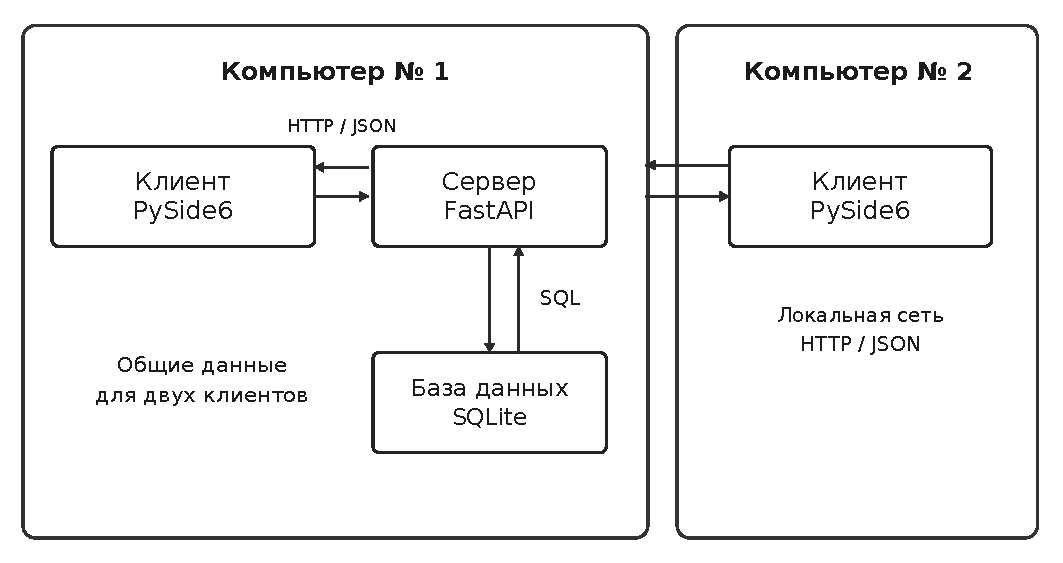
\includegraphics[width=.94\textwidth]{figures/arch.pdf}
\caption{Взаимодействие двух клиентов, сервера и базы данных}
\label{fig:architecture}
\end{figure}

Действие пользователя проходит несколько этапов. Например, при добавлении задачи клиент получает текст из поля ввода. Если введены только пробелы, сообщение об ошибке показывается сразу, без обращения к серверу. Если ввод корректный, клиент отправляет POST-запрос. Сервер ещё раз проверяет название, выполняет вставку в SQLite, сохраняет изменение и отправляет ответ об успехе. После ответа клиент запрашивает обновлённый список. Второй компьютер увидит эту запись после следующего запроса обновления.

При изменении состояния сначала выбирается конкретная строка. Из её данных извлекается целочисленный идентификатор, а затем отправляется PATCH-запрос по её идентификатору. Сервер переключает отметку выполнения соответствующей записи. Если запись уже отсутствует, сервер возвращает HTTP 404. Клиент показывает предупреждение «Не удалось выполнить действие» и повторно запрашивает список. Тот же принцип используется при удалении: операция выполняется только для существующего идентификатора. Смысл используемых методов и кодов ответа соответствует общим правилам HTTP \cite{rfchttp}.

Для синхронизации выбран периодический опрос сервера. В каждом клиенте таймер срабатывает один раз в две секунды и запускает получение списка задач. Полученный список сравнивается с предыдущим. Если изменений нет, интерфейс остаётся таким же. Если данные отличаются, список заполняется заново. Применение таймера для периодических действий предусмотрено библиотекой Qt \cite{qtimer}. Постоянное соединение с сервером для этого алгоритма не используется.

Изменение появляется на втором ПК при следующем запросе таймера, поэтому обновление не происходит мгновенно. Если компьютер-сервер недоступен, клиент показывает ошибку и не сохраняет отправленную команду локально. После восстановления соединения очередной запрос возвращает актуальный список SQLite. Измерение оптимального интервала опроса не проводилось.

При одновременной работе двух пользователей возможны ситуации, когда один удаляет задачу, а второй пытается изменить её состояние. Проверка количества изменённых строк на сервере позволяет отличить несуществующую запись от существующей. В таком случае клиент получает 404. Правила сложного разрешения конфликтов не требуются: все изменения проходят через одну таблицу и выполняются как отдельные операции. Но приложение не фиксирует историю действий, поэтому после удаления нельзя восстановить прежнее состояние средствами самой программы.

\section{Структура базы данных и интерфейса}

Задачи хранятся в таблице \texttt{tasks}. В неё входят идентификатор, название, отметка выполнения. Идентификатор формируется автоматически и позволяет выбрать нужную запись при изменении или удалении. Название хранится как текст. Признак выполнения записывается как число 0 или 1, но в передаваемом JSON преобразуется в логическое значение. Отдельного поля владельца задачи нет, поскольку список общий.

SQLite позволяет создавать таблицу с первичным ключом и ограничениями на отсутствие значения NULL. В таблице нет внешних ключей: каждая запись содержит все данные, необходимые клиенту. Операция создания таблицы выполняется при запуске сервера, причём используется вариант с проверкой существования таблицы. Если файл базы уже содержит данные, повторный запуск не должен удалять их. Синтаксис создания таблицы и назначение первичного ключа описаны в документации SQLite \cite{sqlitecreate}. Состав полей приведён в таблице \ref{tab:dbfields}.

\begin{table}[H]
\caption{Поля таблицы tasks и их смысл}
\label{tab:dbfields}
\small\centering\renewcommand{\arraystretch}{1.25}
\begin{tabularx}{\textwidth}{|L{25mm}|L{33mm}|Y|}
\hline
Поле & Тип & Назначение \\
\hline
id & INTEGER & Уникальный идентификатор записи \\
\hline
title & TEXT & Краткое название задачи \\
\hline
done & INTEGER & 0: в работе, 1: выполнено \\
\hline
\end{tabularx}
\end{table}

Для чтения списка сервер использует запрос SELECT с сортировкой. Новые записи выводятся выше старых, независимо от отметки выполнения. Это правило применяется сервером, поэтому оба клиента получают одинаковый порядок. SQL-операция SELECT предназначена для выбора данных из таблиц и допускает указание порядка результатов \cite{pythonsqlite}.

Изменение состояния выполняется операцией UPDATE, которая меняет поле \texttt{done} только у строки с указанным идентификатором \cite{pythonsqlite}. Удаление реализуется операцией DELETE с таким же условием выбора одной записи \cite{pythonsqlite}. Пользовательский текст передаётся в SQL как параметр, что позволяет безопасно хранить обычные символы, включая кавычки. В коде нет ручного построения SQL-запроса из введённого названия.

В клиенте три страницы (рисунок \ref{fig:navigation}). На первой доступны добавление, поиск, фильтрация, редактирование, изменение статуса, удаление и сохранение списка в TXT. На второй показаны число всех задач, количество выполненных и индикатор доли выполнения. Третья содержит сведения о программе и адрес сервера. Переключение выполняется вкладками в верхней части окна.

\begin{figure}[htbp]
\centering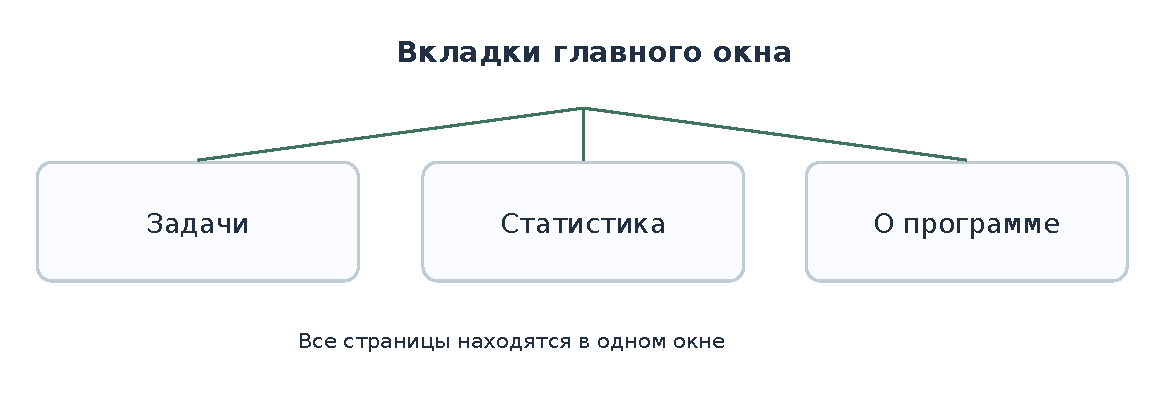
\includegraphics[width=.92\textwidth]{figures/nav.pdf}
\caption{Переход между страницами приложения}
\label{fig:navigation}
\end{figure}

Для переключения трёх страниц используется QTabWidget \cite{qttabs}. Список построен на QListWidget: у каждой строки отдельно сохраняется идентификатор задачи. Кнопка «Изменить» открывает стандартный диалог ввода текста; двойной щелчок по строке меняет отметку выполнения \cite{qtlist}. Поиск сравнивает названия без учёта регистра, а фильтр оставляет все задачи, только невыполненные или только выполненные.

В памяти клиента хранится последний полученный список задач. Это позволяет не перестраивать список каждые две секунды без необходимости. При обновлении, которое действительно меняет строки, клиент пытается сохранить выбранную пользователем запись по её идентификатору. Такой механизм нужен, чтобы автоматический опрос не мешал нажимать кнопки. Данные о выбранной строке читаются из специального поля элемента списка, а не извлекаются из видимого текста, который может совпадать у разных задач.

Страница статистики показывает общее число задач, количество выполненных и их процент. Если список пуст, индикатор показывает ноль. Эти показатели вычисляются из полученных клиентом данных, без дополнительных таблиц и запросов к базе. Адрес сервера задаётся при запуске клиента, а не через отдельную страницу настроек.
